\documentclass[twoside]{book}

% Packages required by doxygen
\usepackage{fixltx2e}
\usepackage{calc}
\usepackage{doxygen}
\usepackage{graphicx}
\usepackage[utf8]{inputenc}
\usepackage{makeidx}
\usepackage{multicol}
\usepackage{multirow}
\PassOptionsToPackage{warn}{textcomp}
\usepackage{textcomp}
\usepackage[nointegrals]{wasysym}
\usepackage[table]{xcolor}

% Font selection
\usepackage[T1]{fontenc}
\usepackage{mathptmx}
\usepackage[scaled=.90]{helvet}
\usepackage{courier}
\usepackage{amssymb}
\usepackage{sectsty}
\renewcommand{\familydefault}{\sfdefault}
\allsectionsfont{%
  \fontseries{bc}\selectfont%
  \color{darkgray}%
}
\renewcommand{\DoxyLabelFont}{%
  \fontseries{bc}\selectfont%
  \color{darkgray}%
}
\newcommand{\+}{\discretionary{\mbox{\scriptsize$\hookleftarrow$}}{}{}}

% Page & text layout
\usepackage{geometry}
\geometry{%
  a4paper,%
  top=2.5cm,%
  bottom=2.5cm,%
  left=2.5cm,%
  right=2.5cm%
}
\tolerance=750
\hfuzz=15pt
\hbadness=750
\setlength{\emergencystretch}{15pt}
\setlength{\parindent}{0cm}
\setlength{\parskip}{0.2cm}
\makeatletter
\renewcommand{\paragraph}{%
  \@startsection{paragraph}{4}{0ex}{-1.0ex}{1.0ex}{%
    \normalfont\normalsize\bfseries\SS@parafont%
  }%
}
\renewcommand{\subparagraph}{%
  \@startsection{subparagraph}{5}{0ex}{-1.0ex}{1.0ex}{%
    \normalfont\normalsize\bfseries\SS@subparafont%
  }%
}
\makeatother

% Headers & footers
\usepackage{fancyhdr}
\pagestyle{fancyplain}
\fancyhead[LE]{\fancyplain{}{\bfseries\thepage}}
\fancyhead[CE]{\fancyplain{}{}}
\fancyhead[RE]{\fancyplain{}{\bfseries\leftmark}}
\fancyhead[LO]{\fancyplain{}{\bfseries\rightmark}}
\fancyhead[CO]{\fancyplain{}{}}
\fancyhead[RO]{\fancyplain{}{\bfseries\thepage}}
\fancyfoot[LE]{\fancyplain{}{}}
\fancyfoot[CE]{\fancyplain{}{}}
\fancyfoot[RE]{\fancyplain{}{\bfseries\scriptsize Generated on Wed Aug 24 2016 05\+:25\+:54 for bsz7\+\_\+robocup by Doxygen }}
\fancyfoot[LO]{\fancyplain{}{\bfseries\scriptsize Generated on Wed Aug 24 2016 05\+:25\+:54 for bsz7\+\_\+robocup by Doxygen }}
\fancyfoot[CO]{\fancyplain{}{}}
\fancyfoot[RO]{\fancyplain{}{}}
\renewcommand{\footrulewidth}{0.4pt}
\renewcommand{\chaptermark}[1]{%
  \markboth{#1}{}%
}
\renewcommand{\sectionmark}[1]{%
  \markright{\thesection\ #1}%
}

% Indices & bibliography
\usepackage{natbib}
\usepackage[titles]{tocloft}
\setcounter{tocdepth}{3}
\setcounter{secnumdepth}{5}
\makeindex

% Hyperlinks (required, but should be loaded last)
\usepackage{ifpdf}
\ifpdf
  \usepackage[pdftex,pagebackref=true]{hyperref}
\else
  \usepackage[ps2pdf,pagebackref=true]{hyperref}
\fi
\hypersetup{%
  colorlinks=true,%
  linkcolor=blue,%
  citecolor=blue,%
  unicode%
}

% Custom commands
\newcommand{\clearemptydoublepage}{%
  \newpage{\pagestyle{empty}\cleardoublepage}%
}


%===== C O N T E N T S =====

\begin{document}

% Titlepage & ToC
\hypersetup{pageanchor=false,
             bookmarks=true,
             bookmarksnumbered=true,
             pdfencoding=unicode
            }
\pagenumbering{roman}
\begin{titlepage}
\vspace*{7cm}
\begin{center}%
{\Large bsz7\+\_\+robocup \\[1ex]\large 0.\+1 }\\
\vspace*{1cm}
{\large Generated by Doxygen 1.8.8}\\
\vspace*{0.5cm}
{\small Wed Aug 24 2016 05:25:54}\\
\end{center}
\end{titlepage}
\clearemptydoublepage
\tableofcontents
\clearemptydoublepage
\pagenumbering{arabic}
\hypersetup{pageanchor=true}

%--- Begin generated contents ---
\chapter{Hierarchical Index}
\section{Class Hierarchy}
This inheritance list is sorted roughly, but not completely, alphabetically\+:\begin{DoxyCompactList}
\item \contentsline{section}{rc\+:\+:Blob\+Detector}{\pageref{classrc_1_1BlobDetector}}{}
\begin{DoxyCompactList}
\item \contentsline{section}{rc\+:\+:Blob\+Detector\+Factory}{\pageref{classrc_1_1BlobDetectorFactory}}{}
\end{DoxyCompactList}
\item \contentsline{section}{rc\+:\+:cb\+Element$<$ T $>$}{\pageref{structrc_1_1cbElement}}{}
\item \contentsline{section}{rc\+:\+:cb\+Element$<$ cv\+:\+:Mat $>$}{\pageref{structrc_1_1cbElement}}{}
\item \contentsline{section}{rc\+:\+:Circular\+Buffer$<$ T $>$}{\pageref{classrc_1_1CircularBuffer}}{}
\item \contentsline{section}{rc\+:\+:Circular\+Buffer$<$ cv\+:\+:Mat $>$}{\pageref{classrc_1_1CircularBuffer}}{}
\begin{DoxyCompactList}
\item \contentsline{section}{rc\+:\+:Camera}{\pageref{classrc_1_1Camera}}{}
\begin{DoxyCompactList}
\item \contentsline{section}{rc\+:\+:Blob\+Detector\+Factory}{\pageref{classrc_1_1BlobDetectorFactory}}{}
\end{DoxyCompactList}
\end{DoxyCompactList}
\item \contentsline{section}{cmd\+\_\+opts}{\pageref{structcmd__opts}}{}
\item \contentsline{section}{rc\+:\+:Daemon}{\pageref{classrc_1_1Daemon}}{}
\item \contentsline{section}{rc\+:\+:image\+Obj}{\pageref{structrc_1_1imageObj}}{}
\item Raspi\+Cam\+\_\+\+Cv\begin{DoxyCompactList}
\item \contentsline{section}{rc\+:\+:Camera}{\pageref{classrc_1_1Camera}}{}
\end{DoxyCompactList}
\item \contentsline{section}{rc\+:\+:Semaphore}{\pageref{classrc_1_1Semaphore}}{}
\item \contentsline{section}{rc\+:\+:Window}{\pageref{classrc_1_1Window}}{}
\end{DoxyCompactList}

\chapter{Class Index}
\section{Class List}
Here are the classes, structs, unions and interfaces with brief descriptions\+:\begin{DoxyCompactList}
\item\contentsline{section}{\hyperlink{classrc_1_1Camera}{rc\+::\+Camera} }{\pageref{classrc_1_1Camera}}{}
\item\contentsline{section}{\hyperlink{structrc_1_1cbElement}{rc\+::cb\+Element$<$ T $>$} }{\pageref{structrc_1_1cbElement}}{}
\item\contentsline{section}{\hyperlink{classrc_1_1CircularBuffer}{rc\+::\+Circular\+Buffer$<$ T $>$} }{\pageref{classrc_1_1CircularBuffer}}{}
\item\contentsline{section}{\hyperlink{structcmd__opts}{cmd\+\_\+opts} }{\pageref{structcmd__opts}}{}
\item\contentsline{section}{\hyperlink{classrc_1_1Daemon}{rc\+::\+Daemon} }{\pageref{classrc_1_1Daemon}}{}
\item\contentsline{section}{\hyperlink{classrc_1_1Detector}{rc\+::\+Detector} }{\pageref{classrc_1_1Detector}}{}
\item\contentsline{section}{\hyperlink{classrc_1_1DetectorFactory}{rc\+::\+Detector\+Factory} }{\pageref{classrc_1_1DetectorFactory}}{}
\item\contentsline{section}{\hyperlink{structrc_1_1processed__image}{rc\+::processed\+\_\+image} }{\pageref{structrc_1_1processed__image}}{}
\item\contentsline{section}{\hyperlink{structrc_1_1threadData}{rc\+::thread\+Data} }{\pageref{structrc_1_1threadData}}{}
\item\contentsline{section}{\hyperlink{classrc_1_1Threads}{rc\+::\+Threads} }{\pageref{classrc_1_1Threads}}{}
\item\contentsline{section}{\hyperlink{structrc_1_1time__consumption}{rc\+::time\+\_\+consumption} }{\pageref{structrc_1_1time__consumption}}{}
\item\contentsline{section}{\hyperlink{classrc_1_1WebServer}{rc\+::\+Web\+Server} }{\pageref{classrc_1_1WebServer}}{}
\item\contentsline{section}{\hyperlink{classrc_1_1Window}{rc\+::\+Window} }{\pageref{classrc_1_1Window}}{}
\end{DoxyCompactList}

\chapter{File Index}
\section{File List}
Here is a list of all documented files with brief descriptions\+:\begin{DoxyCompactList}
\item\contentsline{section}{src/\hyperlink{RC__BlobDetector_8hpp}{R\+C\+\_\+\+Blob\+Detector.\+hpp} }{\pageref{RC__BlobDetector_8hpp}}{}
\item\contentsline{section}{src/\hyperlink{RC__BlobDetectorFactory_8hpp}{R\+C\+\_\+\+Blob\+Detector\+Factory.\+hpp} }{\pageref{RC__BlobDetectorFactory_8hpp}}{}
\item\contentsline{section}{src/\hyperlink{RC__Camera_8hpp}{R\+C\+\_\+\+Camera.\+hpp} \\*Eine Klasse zur Steuerung der Kamera und des Zwischenspeichers (Puffer) }{\pageref{RC__Camera_8hpp}}{}
\item\contentsline{section}{src/\hyperlink{RC__CircularBuffer_8hpp}{R\+C\+\_\+\+Circular\+Buffer.\+hpp} }{\pageref{RC__CircularBuffer_8hpp}}{}
\item\contentsline{section}{src/\hyperlink{RC__Daemon_8hpp}{R\+C\+\_\+\+Daemon.\+hpp} }{\pageref{RC__Daemon_8hpp}}{}
\item\contentsline{section}{src/\hyperlink{RC__Main_8cpp}{R\+C\+\_\+\+Main.\+cpp} \\*Initialisierung, Parameter auswerten, Einstellungen setzen }{\pageref{RC__Main_8cpp}}{}
\item\contentsline{section}{src/\hyperlink{RC__Semaphore_8hpp}{R\+C\+\_\+\+Semaphore.\+hpp} }{\pageref{RC__Semaphore_8hpp}}{}
\item\contentsline{section}{src/\hyperlink{RC__WebServer_8hpp}{R\+C\+\_\+\+Web\+Server.\+hpp} }{\pageref{RC__WebServer_8hpp}}{}
\item\contentsline{section}{src/\hyperlink{RC__Window_8hpp}{R\+C\+\_\+\+Window.\+hpp} }{\pageref{RC__Window_8hpp}}{}
\end{DoxyCompactList}

\chapter{Class Documentation}
\hypertarget{classrc_1_1BlobDetector}{\section{rc\+:\+:Blob\+Detector Class Reference}
\label{classrc_1_1BlobDetector}\index{rc\+::\+Blob\+Detector@{rc\+::\+Blob\+Detector}}
}
Inheritance diagram for rc\+:\+:Blob\+Detector\+:\begin{figure}[H]
\begin{center}
\leavevmode
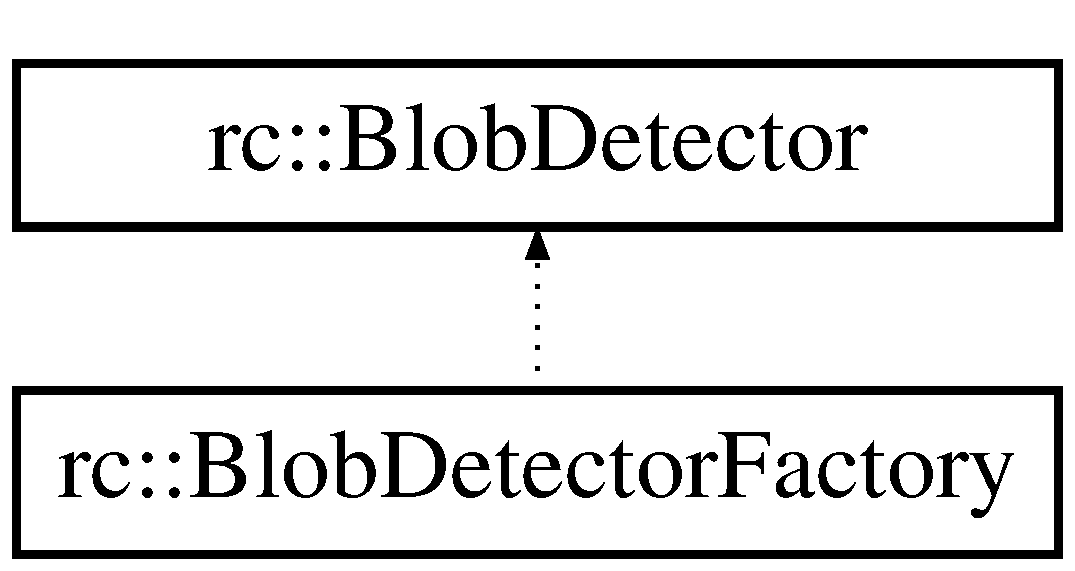
\includegraphics[height=2.000000cm]{classrc_1_1BlobDetector}
\end{center}
\end{figure}
\subsection*{Public Member Functions}
\begin{Indent}{\bf Konstruktor}\par
\begin{DoxyCompactItemize}
\item 
\hypertarget{classrc_1_1BlobDetector_af7e4f2625974457c6949970d6bdd25dd}{{\bfseries Blob\+Detector} ()}\label{classrc_1_1BlobDetector_af7e4f2625974457c6949970d6bdd25dd}

\end{DoxyCompactItemize}
\end{Indent}
\begin{Indent}{\bf Destruktor}\par
\begin{DoxyCompactItemize}
\item 
\hypertarget{classrc_1_1BlobDetector_a39ef0b4e8945d64e9348923a8cf57377}{{\bfseries $\sim$\+Blob\+Detector} ()}\label{classrc_1_1BlobDetector_a39ef0b4e8945d64e9348923a8cf57377}

\end{DoxyCompactItemize}
\end{Indent}
\begin{Indent}{\bf Farbfilter}\par
{\em 
\begin{DoxyParams}{Parameters}
{\em Quellbild} & \\
\hline
{\em zu} & filternde Farbe \\
\hline
\end{DoxyParams}

\begin{DoxyRetVals}{Return values}
{\em die} & gefilterte Open\+C\+V Matrix \\
\hline
\end{DoxyRetVals}
}\begin{DoxyCompactItemize}
\item 
\hypertarget{classrc_1_1BlobDetector_a1bec455c6bf7d4d8b2ae7c114320a8f1}{cv\+::\+Mat {\bfseries filter\+Color} (cv\+::\+Mat src, enum robo\+Color rcol)}\label{classrc_1_1BlobDetector_a1bec455c6bf7d4d8b2ae7c114320a8f1}

\end{DoxyCompactItemize}
\end{Indent}
\begin{Indent}{\bf Sucht nach Konturen in einem Bild}\par
{\em 
\begin{DoxyParams}{Parameters}
{\em Das} & zu filternde Bild. \\
\hline
{\em die} & zu filternde Farbe \\
\hline
{\em ausgewertete} & Informationen in dieser Struktur speichern \\
\hline
\end{DoxyParams}

\begin{DoxyRetVals}{Return values}
{\em Matrix} & nach dem Farbfilter \\
\hline
\end{DoxyRetVals}
}\begin{DoxyCompactItemize}
\item 
\hypertarget{classrc_1_1BlobDetector_a90e6fd34936395a7bd338665cb3c3d2a}{cv\+::\+Mat {\bfseries process} (cv\+::\+Mat \&image, enum robo\+Color rc, struct \hyperlink{structrc_1_1processed__image}{processed\+\_\+image} $\ast$pi)}\label{classrc_1_1BlobDetector_a90e6fd34936395a7bd338665cb3c3d2a}

\end{DoxyCompactItemize}
\end{Indent}


The documentation for this class was generated from the following files\+:\begin{DoxyCompactItemize}
\item 
src/\hyperlink{RC__BlobDetector_8hpp}{R\+C\+\_\+\+Blob\+Detector.\+hpp}\item 
src/R\+C\+\_\+\+Blob\+Detector.\+cpp\end{DoxyCompactItemize}

\hypertarget{classrc_1_1BlobDetectorFactory}{\section{rc\+:\+:Blob\+Detector\+Factory Class Reference}
\label{classrc_1_1BlobDetectorFactory}\index{rc\+::\+Blob\+Detector\+Factory@{rc\+::\+Blob\+Detector\+Factory}}
}
Inheritance diagram for rc\+:\+:Blob\+Detector\+Factory\+:\begin{figure}[H]
\begin{center}
\leavevmode
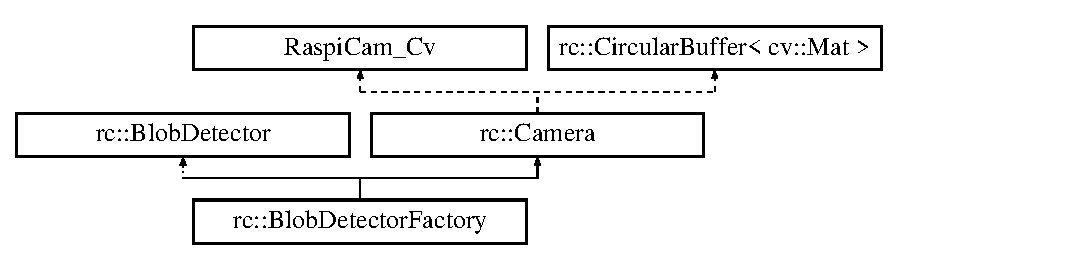
\includegraphics[height=3.000000cm]{classrc_1_1BlobDetectorFactory}
\end{center}
\end{figure}
\subsection*{Public Member Functions}
\begin{Indent}{\bf Konstruktor}\par
{\em 
\begin{DoxyParams}[1]{Parameters}
\mbox{\tt in}  & {\em Anzahl} & der zu \char`\"{}\+Arbeiter\char`\"{}-\/ Threads \\
\hline
\end{DoxyParams}
}\begin{DoxyCompactItemize}
\item 
\hypertarget{classrc_1_1BlobDetectorFactory_ad23d95cfe5c4a4204b5e1fc38c62dc8a}{{\bfseries Blob\+Detector\+Factory} (unsigned int num\+Threads)}\label{classrc_1_1BlobDetectorFactory_ad23d95cfe5c4a4204b5e1fc38c62dc8a}

\end{DoxyCompactItemize}
\end{Indent}
\begin{Indent}{\bf Standart Destruktor}\par
\begin{DoxyCompactItemize}
\item 
\hypertarget{classrc_1_1BlobDetectorFactory_a5532ab9249a1c53c4b87a968be4d6235}{{\bfseries $\sim$\+Blob\+Detector\+Factory} ()}\label{classrc_1_1BlobDetectorFactory_a5532ab9249a1c53c4b87a968be4d6235}

\end{DoxyCompactItemize}
\end{Indent}
\begin{Indent}{\bf Initialisierung der Kamera}\par
{\em Hinweis\+: Diese Methode sollte {\itshape vor} start\+Threads() ausgeführt werden }\begin{DoxyCompactItemize}
\item 
\hypertarget{classrc_1_1BlobDetectorFactory_a8816a3c768cde4d4491f2ab06f875df3}{bool {\bfseries open\+Camera} (void)}\label{classrc_1_1BlobDetectorFactory_a8816a3c768cde4d4491f2ab06f875df3}

\end{DoxyCompactItemize}
\end{Indent}
\begin{Indent}{\bf Deaktiviert die Kamera}\par
{\em Hinweis\+: Diese Methode sollte {\itshape nach} stop\+Threads() ausgeführt werden }\begin{DoxyCompactItemize}
\item 
\hypertarget{classrc_1_1BlobDetectorFactory_a847250d92a85518c9701ab8152c542f5}{void {\bfseries close\+Camera} (void)}\label{classrc_1_1BlobDetectorFactory_a847250d92a85518c9701ab8152c542f5}

\end{DoxyCompactItemize}
\end{Indent}
\begin{Indent}{\bf Startet die \char`\"{}\+Arbeiter\char`\"{}-\/ Threads}\par
{\em Die Threads werden gestartet und befinden sich in einer Endlosschleife, solange das Programm nicht beendet wird oder stop\+Threads() aufgerufen wird. }\begin{DoxyCompactItemize}
\item 
\hypertarget{classrc_1_1BlobDetectorFactory_afecac9963fc4e69e51422ce59cf540f3}{void {\bfseries start\+Threads} (void)}\label{classrc_1_1BlobDetectorFactory_afecac9963fc4e69e51422ce59cf540f3}

\end{DoxyCompactItemize}
\end{Indent}
\begin{Indent}{\bf Stoppt alle \char`\"{}\+Arbeiter\char`\"{}-\/ Threads}\par
{\em Alle Threads werden beendet. Erst nachdem alle Threads beendet wurden, kerht diese Methode zum aufrufenden zurück. }\begin{DoxyCompactItemize}
\item 
\hypertarget{classrc_1_1BlobDetectorFactory_a9dc44508f5a3dd4beaee0813b7443194}{void {\bfseries stop\+Threads} (void)}\label{classrc_1_1BlobDetectorFactory_a9dc44508f5a3dd4beaee0813b7443194}

\end{DoxyCompactItemize}
\end{Indent}
\begin{Indent}{\bf Gibt Informationen über diese Klasse als String zurück.}\par
{\em Dabei werden Informationen über den \hyperlink{classrc_1_1CircularBuffer}{Circular\+Buffer} und der Window-\/ Klasse ausgegeben.

\begin{DoxyReturn}{Returns}
Die Informationen als Zeichenkette. 
\end{DoxyReturn}
}\begin{DoxyCompactItemize}
\item 
\hypertarget{classrc_1_1BlobDetectorFactory_a08e56c167bd2f928d2f808d429d8327e}{std\+::string {\bfseries out\+Info} (void)}\label{classrc_1_1BlobDetectorFactory_a08e56c167bd2f928d2f808d429d8327e}

\end{DoxyCompactItemize}
\end{Indent}
\subsection*{Setzt die Groese des Vorschau-\/ Videos.}
\label{_amgrp31fff75453dbcfb0cbda6f83097f2790}%
Dabei ist zu beachten, dass die moeglichst kleine Werte gewaehlt werden sollten, um den Raspberry nicht zu ueberlasten.


\begin{DoxyParams}{Parameters}
{\em Breite} & in Pixel \\
\hline
{\em Hoehe} & in Pixel \\
\hline
\end{DoxyParams}
\begin{DoxyCompactItemize}
\item 
\hypertarget{classrc_1_1BlobDetectorFactory_a4bf955ad08f9218729777737b9071e35}{void {\bfseries set\+Dimensions} (unsigned int width, unsigned int height)}\label{classrc_1_1BlobDetectorFactory_a4bf955ad08f9218729777737b9071e35}

\end{DoxyCompactItemize}
\subsection*{Additional Inherited Members}


The documentation for this class was generated from the following files\+:\begin{DoxyCompactItemize}
\item 
src/\hyperlink{RC__BlobDetectorFactory_8hpp}{R\+C\+\_\+\+Blob\+Detector\+Factory.\+hpp}\item 
src/R\+C\+\_\+\+Blob\+Detector\+Factory.\+cpp\end{DoxyCompactItemize}

\hypertarget{classrc_1_1Camera}{\section{rc\+:\+:Camera Class Reference}
\label{classrc_1_1Camera}\index{rc\+::\+Camera@{rc\+::\+Camera}}
}
Inheritance diagram for rc\+:\+:Camera\+:\begin{figure}[H]
\begin{center}
\leavevmode
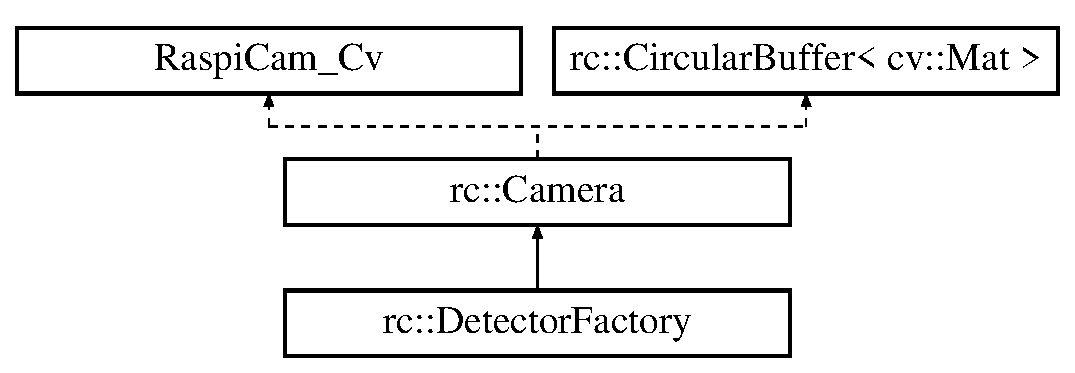
\includegraphics[height=3.000000cm]{classrc_1_1Camera}
\end{center}
\end{figure}
\subsection*{Public Member Functions}
\begin{Indent}{\bf Kamera Konstruktor}\par
{\em 
\begin{DoxyParams}[1]{Parameters}
\mbox{\tt in}  & {\em max\+Buffer\+Elements} & größe des Pufferspeichers (\hyperlink{classrc_1_1CircularBuffer}{rc\+::\+Circular\+Buffer}) \\
\hline
\end{DoxyParams}

\begin{DoxyRetVals}{Return values}
{\em Kamera} & Objekt \\
\hline
\end{DoxyRetVals}
}\begin{DoxyCompactItemize}
\item 
\hypertarget{classrc_1_1Camera_aefbf57e5308b3e72aeabe7b0308c1d93}{{\bfseries Camera} (unsigned int max\+Buffer\+Elements)}\label{classrc_1_1Camera_aefbf57e5308b3e72aeabe7b0308c1d93}

\end{DoxyCompactItemize}
\end{Indent}
\begin{Indent}{\bf Standart Destruktor}\par
{\em Dieser ist z.\+Z. ausreichend, da keine \char`\"{}aufräum\char`\"{}-\/ Arbeiten nötig sind. }\begin{DoxyCompactItemize}
\item 
\hypertarget{classrc_1_1Camera_ad219ec460144ffc914e10250fef89677}{{\bfseries $\sim$\+Camera} (void)}\label{classrc_1_1Camera_ad219ec460144ffc914e10250fef89677}

\end{DoxyCompactItemize}
\end{Indent}
\begin{Indent}{\bf Kamerabild holen}\par
{\em Ein Kamerabild \char`\"{}grabschen\char`\"{}.


\begin{DoxyRetVals}{Return values}
{\em T\+R\+U\+E} & Kamerabild konnte erfolgreich geholt werden \\
\hline
{\em F\+A\+L\+S\+E} & entweder lieferte die Kamera kein bild oder der Pufferspeicher ist voll\\
\hline
\end{DoxyRetVals}
Wichtig\+: Damit ein Bild von der Kamera geholt werden kann, muss vorher raspicam\+::\+Raspi\+Cam\+\_\+\+Cv\+::open() aufgerugen werden! }\begin{DoxyCompactItemize}
\item 
\hypertarget{classrc_1_1Camera_a5d8610c2bbebbc9cd7a56e00549b514c}{bool {\bfseries grab\+Camera\+Image} (void)}\label{classrc_1_1Camera_a5d8610c2bbebbc9cd7a56e00549b514c}

\end{DoxyCompactItemize}
\end{Indent}
\begin{Indent}{\bf Breite eines Kamerabildes zurückgeben}\par
{\em 
\begin{DoxyRetVals}{Return values}
{\em die} & Breite in Pixel \\
\hline
\end{DoxyRetVals}
}\begin{DoxyCompactItemize}
\item 
\hypertarget{classrc_1_1Camera_a1260f90780be36eb52db9f90d73578e9}{unsigned int {\bfseries get\+Width} (void)}\label{classrc_1_1Camera_a1260f90780be36eb52db9f90d73578e9}

\end{DoxyCompactItemize}
\end{Indent}
\begin{Indent}{\bf Höhe eines Kamerabildes zurückgeben}\par
{\em 
\begin{DoxyRetVals}{Return values}
{\em die} & Höhe in Pixel \\
\hline
\end{DoxyRetVals}
}\begin{DoxyCompactItemize}
\item 
\hypertarget{classrc_1_1Camera_a3a279a087aa5864793aa9c5628bea40a}{unsigned int {\bfseries get\+Height} (void)}\label{classrc_1_1Camera_a3a279a087aa5864793aa9c5628bea40a}

\end{DoxyCompactItemize}
\end{Indent}
\begin{Indent}{\bf Breite eines Kamerabildes festlegen}\par
{\em 
\begin{DoxyParams}{Parameters}
{\em die} & Breite in Pixel \\
\hline
\end{DoxyParams}
}\begin{DoxyCompactItemize}
\item 
\hypertarget{classrc_1_1Camera_a7f45f935fa50f95f78d1d2a3629f2a91}{void {\bfseries set\+Width} (unsigned int width)}\label{classrc_1_1Camera_a7f45f935fa50f95f78d1d2a3629f2a91}

\end{DoxyCompactItemize}
\end{Indent}
\begin{Indent}{\bf Höhe eines Kamerabildes festlegen}\par
{\em 
\begin{DoxyParams}{Parameters}
{\em die} & Höhe in Pixel \\
\hline
\end{DoxyParams}
}\begin{DoxyCompactItemize}
\item 
\hypertarget{classrc_1_1Camera_aeea452211d9fec8761c6aaa7bbb6d5ea}{void {\bfseries set\+Height} (unsigned int height)}\label{classrc_1_1Camera_aeea452211d9fec8761c6aaa7bbb6d5ea}

\end{DoxyCompactItemize}
\end{Indent}
\begin{Indent}{\bf Format der Kamerabilder zurückgeben}\par
{\em 
\begin{DoxyRetVals}{Return values}
{\em C\+V\+\_\+8\+U\+C1} & Schwarz-\/\+Weiß (1 Byte Farbabstufung) \\
\hline
{\em C\+V\+\_\+8\+U\+C3} & Farbe (3 Byte pro Kanal -\/$>$ R\+G\+B) \\
\hline
\end{DoxyRetVals}
}\begin{DoxyCompactItemize}
\item 
\hypertarget{classrc_1_1Camera_aa0cd8c29ec174d184ddcd78084258026}{raspicam\+::\+R\+A\+S\+P\+I\+C\+A\+M\+\_\+\+F\+O\+R\+M\+A\+T {\bfseries get\+Format} (void)}\label{classrc_1_1Camera_aa0cd8c29ec174d184ddcd78084258026}

\end{DoxyCompactItemize}
\end{Indent}
\begin{Indent}{\bf Farbsättigung zurückgeben}\par
{\em 
\begin{DoxyRetVals}{Return values}
{\em ein} & Wert zwischen 0 (keine Sättigung) und 100 (volle Sättigung) \\
\hline
\end{DoxyRetVals}
}\begin{DoxyCompactItemize}
\item 
\hypertarget{classrc_1_1Camera_adf54b48540f83fdcecff277443fbc360}{unsigned int {\bfseries get\+Saturation} (void)}\label{classrc_1_1Camera_adf54b48540f83fdcecff277443fbc360}

\end{DoxyCompactItemize}
\end{Indent}
\begin{Indent}{\bf Bildverstärkung zurückgeben (Treiber spezifisch)}\par
{\em 
\begin{DoxyRetVals}{Return values}
{\em ein} & Wert zwischen 0 (keine Verstärkung) und 100 (maximale Verstärkung) \\
\hline
\end{DoxyRetVals}
}\begin{DoxyCompactItemize}
\item 
\hypertarget{classrc_1_1Camera_aa4f5ffc75180f60ba018f00669bddeee}{unsigned int {\bfseries get\+Gain} (void)}\label{classrc_1_1Camera_aa4f5ffc75180f60ba018f00669bddeee}

\end{DoxyCompactItemize}
\end{Indent}
\begin{Indent}{\bf Belichtungsdauer zurückgeben}\par
{\em 
\begin{DoxyRetVals}{Return values}
{\em ein} & Wert zwischen 1 (kurze Belichtungsdauer) und 100 (lange B\+Elichtungsdauer) oder -\/1 ffür eine automatische Belichtungsdauer \\
\hline
\end{DoxyRetVals}
}\begin{DoxyCompactItemize}
\item 
\hypertarget{classrc_1_1Camera_a6e906a0b175eb28fa1dd4dbab4aa697a}{int {\bfseries get\+Exposure} (void)}\label{classrc_1_1Camera_a6e906a0b175eb28fa1dd4dbab4aa697a}

\end{DoxyCompactItemize}
\end{Indent}
\begin{Indent}{\bf Maximale Anzahl Bilder/\+Sekunde der Kamera}\par
{\em 
\begin{DoxyRetVals}{Return values}
{\em ein} & Wert von 1 bis n \\
\hline
\end{DoxyRetVals}
}\begin{DoxyCompactItemize}
\item 
\hypertarget{classrc_1_1Camera_a1bb66807b50fe1e4e2d3941d266073cf}{unsigned int {\bfseries get\+Max\+F\+P\+S} (void)}\label{classrc_1_1Camera_a1bb66807b50fe1e4e2d3941d266073cf}

\end{DoxyCompactItemize}
\end{Indent}
\begin{Indent}{\bf Sättigung festlegen}\par
{\em 
\begin{DoxyParams}[1]{Parameters}
\mbox{\tt in}  & {\em value} & siehe \\
\hline
\end{DoxyParams}
\begin{DoxySeeAlso}{See also}
rc\+::\+Camera\+::get\+Saturation 
\end{DoxySeeAlso}
}\begin{DoxyCompactItemize}
\item 
\hypertarget{classrc_1_1Camera_ace923daca0f3b491c966630b441a916e}{void {\bfseries set\+Saturation} (unsigned int value)}\label{classrc_1_1Camera_ace923daca0f3b491c966630b441a916e}

\end{DoxyCompactItemize}
\end{Indent}
\begin{Indent}{\bf Bildverstärkung festlegen}\par
{\em 
\begin{DoxyParams}[1]{Parameters}
\mbox{\tt in}  & {\em value} & siehe \\
\hline
\end{DoxyParams}
\begin{DoxySeeAlso}{See also}
rc\+::\+Camera\+::get\+Gain 
\end{DoxySeeAlso}
}\begin{DoxyCompactItemize}
\item 
\hypertarget{classrc_1_1Camera_a3d3a84119c61772d0d8ff06915f41d32}{void {\bfseries set\+Gain} (unsigned int value)}\label{classrc_1_1Camera_a3d3a84119c61772d0d8ff06915f41d32}

\end{DoxyCompactItemize}
\end{Indent}
\begin{Indent}{\bf Belichtungsdauer festlegen}\par
{\em 
\begin{DoxyParams}[1]{Parameters}
\mbox{\tt in}  & {\em value} & siehe \\
\hline
\end{DoxyParams}
\begin{DoxySeeAlso}{See also}
rc\+::\+Camera\+::get\+Exposure 
\end{DoxySeeAlso}
}\begin{DoxyCompactItemize}
\item 
\hypertarget{classrc_1_1Camera_a35859a25c12b6ffe3b48f963f8b350ae}{void {\bfseries set\+Exposure} (int value)}\label{classrc_1_1Camera_a35859a25c12b6ffe3b48f963f8b350ae}

\end{DoxyCompactItemize}
\end{Indent}
\begin{Indent}{\bf Maximale Bilder/\+Sekunde setzen}\par
{\em 
\begin{DoxyParams}[1]{Parameters}
\mbox{\tt in}  & {\em value} & siehe \\
\hline
\end{DoxyParams}
\begin{DoxySeeAlso}{See also}
rc\+::\+Camera\+::get\+Max\+F\+P\+S 
\end{DoxySeeAlso}
}\begin{DoxyCompactItemize}
\item 
\hypertarget{classrc_1_1Camera_ab95f1bb0c2778beba736ad92e75fb8da}{void {\bfseries set\+Max\+F\+P\+S} (unsigned int value)}\label{classrc_1_1Camera_ab95f1bb0c2778beba736ad92e75fb8da}

\end{DoxyCompactItemize}
\end{Indent}
\subsection*{Additional Inherited Members}


The documentation for this class was generated from the following files\+:\begin{DoxyCompactItemize}
\item 
src/\hyperlink{RC__Camera_8hpp}{R\+C\+\_\+\+Camera.\+hpp}\item 
src/R\+C\+\_\+\+Camera.\+cpp\end{DoxyCompactItemize}

\hypertarget{structrc_1_1cbElement}{\section{rc\+:\+:cb\+Element$<$ T $>$ Struct Template Reference}
\label{structrc_1_1cbElement}\index{rc\+::cb\+Element$<$ T $>$@{rc\+::cb\+Element$<$ T $>$}}
}
\subsection*{Public Attributes}
\begin{DoxyCompactItemize}
\item 
\hypertarget{structrc_1_1cbElement_a9e0ab0b1cc53698c5aedf11997ffd261}{T {\bfseries element}}\label{structrc_1_1cbElement_a9e0ab0b1cc53698c5aedf11997ffd261}

\item 
\hypertarget{structrc_1_1cbElement_a721d493bd93248172628c48c4526f105}{bool {\bfseries processed}}\label{structrc_1_1cbElement_a721d493bd93248172628c48c4526f105}

\item 
\hypertarget{structrc_1_1cbElement_a101e7ac69a01db74bf72a1a2b768a6d6}{unsigned int {\bfseries id}}\label{structrc_1_1cbElement_a101e7ac69a01db74bf72a1a2b768a6d6}

\end{DoxyCompactItemize}


The documentation for this struct was generated from the following file\+:\begin{DoxyCompactItemize}
\item 
src/R\+C\+\_\+\+Circular\+Buffer.\+hpp\end{DoxyCompactItemize}

\hypertarget{classrc_1_1CircularBuffer}{\section{rc\+:\+:Circular\+Buffer$<$ T $>$ Class Template Reference}
\label{classrc_1_1CircularBuffer}\index{rc\+::\+Circular\+Buffer$<$ T $>$@{rc\+::\+Circular\+Buffer$<$ T $>$}}
}
\subsection*{Public Member Functions}
\begin{Indent}{\bf Konstruktor für zirkulären Pufferspeicher}\par
{\em Anzahl \char`\"{}frischer\char`\"{} Einträge


\begin{DoxyParams}{Parameters}
{\em maximale} & Größe des Pufferspeichers (Anzahl der Elemente) \\
\hline
\end{DoxyParams}
}\begin{DoxyCompactItemize}
\item 
\hypertarget{classrc_1_1CircularBuffer_af0abd0737caf863845860418e36cee61}{{\bfseries Circular\+Buffer} (unsigned int max\+Elements)}\label{classrc_1_1CircularBuffer_af0abd0737caf863845860418e36cee61}

\end{DoxyCompactItemize}
\end{Indent}
\begin{Indent}{\bf Destruktor}\par
\begin{DoxyCompactItemize}
\item 
\hypertarget{classrc_1_1CircularBuffer_a5d0be18eb4de56cacfcc716c55e55639}{{\bfseries $\sim$\+Circular\+Buffer} (void)}\label{classrc_1_1CircularBuffer_a5d0be18eb4de56cacfcc716c55e55639}

\end{DoxyCompactItemize}
\end{Indent}
\begin{Indent}{\bf neues Element dem Pufferspeicher hinzufügen}\par
{\em 
\begin{DoxyParams}{Parameters}
{\em Element} & vom Typ des Templates \\
\hline
\end{DoxyParams}
}\begin{DoxyCompactItemize}
\item 
\hypertarget{classrc_1_1CircularBuffer_aa03a62fe9deae36e5b83200f9f7a2c24}{void {\bfseries add\+Element} (T \&elem)}\label{classrc_1_1CircularBuffer_aa03a62fe9deae36e5b83200f9f7a2c24}

\end{DoxyCompactItemize}
\end{Indent}
\begin{Indent}{\bf maximale Anzahl der Elemente im Pufferspeicher zurückgeben}\par
\begin{DoxyCompactItemize}
\item 
\hypertarget{classrc_1_1CircularBuffer_ae4194d665b35b6a86444f54c759878b7}{unsigned int {\bfseries get\+Max\+Element\+Count} (void)}\label{classrc_1_1CircularBuffer_ae4194d665b35b6a86444f54c759878b7}

\end{DoxyCompactItemize}
\end{Indent}
\begin{Indent}{\bf nächsten \char`\"{}freien\char`\"{} Index zurückgeben}\par
{\em Gibt die nächste \char`\"{}freie\char`\"{} (d.\+h. processed=false) Indexposition im Puffer zurück. }\begin{DoxyCompactItemize}
\item 
\hypertarget{classrc_1_1CircularBuffer_a07d170b88c762967442b90ef2a4848fa}{unsigned int {\bfseries get\+Next\+Index} (void)}\label{classrc_1_1CircularBuffer_a07d170b88c762967442b90ef2a4848fa}

\end{DoxyCompactItemize}
\end{Indent}
\begin{Indent}{\bf Anzahl \char`\"{}freier\char`\"{} (d.\+h. processed=false) Elemente zurückgeben}\par
\begin{DoxyCompactItemize}
\item 
\hypertarget{classrc_1_1CircularBuffer_a1bb2a9a349df4e9b8e213434725c8b8f}{unsigned int {\bfseries get\+Element\+Count} (void)}\label{classrc_1_1CircularBuffer_a1bb2a9a349df4e9b8e213434725c8b8f}

\end{DoxyCompactItemize}
\end{Indent}
\begin{Indent}{\bf Sucht nach dem nächsten \char`\"{}freien\char`\"{} Element}\par
{\em 
\begin{DoxyParams}{Parameters}
{\em eine} & Referenz vom Typ des Templates \\
\hline
\end{DoxyParams}

\begin{DoxyRetVals}{Return values}
{\em true,wenn} & ein freies Element vorhanden, andernfalls false \\
\hline
\end{DoxyRetVals}
}\begin{DoxyCompactItemize}
\item 
\hypertarget{classrc_1_1CircularBuffer_a4ef798c56ada44df67cc4bb5ae1a08eb}{bool {\bfseries get\+Element} (T \&arg)}\label{classrc_1_1CircularBuffer_a4ef798c56ada44df67cc4bb5ae1a08eb}

\end{DoxyCompactItemize}
\end{Indent}


The documentation for this class was generated from the following files\+:\begin{DoxyCompactItemize}
\item 
src/\hyperlink{RC__CircularBuffer_8hpp}{R\+C\+\_\+\+Circular\+Buffer.\+hpp}\item 
src/R\+C\+\_\+\+Circular\+Buffer.\+cpp\end{DoxyCompactItemize}

\hypertarget{structcmd__opts}{\section{cmd\+\_\+opts Struct Reference}
\label{structcmd__opts}\index{cmd\+\_\+opts@{cmd\+\_\+opts}}
}
\subsection*{Public Attributes}
\begin{DoxyCompactItemize}
\item 
\hypertarget{structcmd__opts_a0e94dcdbf5c755d97477c346ece96a2e}{bool {\bfseries daemonize}}\label{structcmd__opts_a0e94dcdbf5c755d97477c346ece96a2e}

\item 
unsigned long long int \hyperlink{structcmd__opts_a582f29b5e8c3328779e88bcb22ff3c2e}{count}
\item 
char $\ast$ \hyperlink{structcmd__opts_acee5a1c6793898bbda38d6d7fb5de431}{video\+File}
\item 
bool \hyperlink{structcmd__opts_aee44e8161de659e8fff50e09100f9ada}{use\+X\+Window}
\item 
unsigned int \hyperlink{structcmd__opts_a0f13b6290e7e33c22a258c11ed23f72f}{width}
\item 
unsigned int \hyperlink{structcmd__opts_a0ab9c9cf886559f8cf19dd2f7be072fb}{height}
\item 
unsigned int \hyperlink{structcmd__opts_a2b42f4e7bd954f5ac87c82e9d19a9b84}{max\+Fps}
\item 
uint8\+\_\+t \hyperlink{structcmd__opts_aa83f2910f6a1803ee8c9f9e3581db314}{sat}
\item 
uint8\+\_\+t \hyperlink{structcmd__opts_a55323cae5dfbafe672e6581da99985b9}{gain}
\item 
int8\+\_\+t \hyperlink{structcmd__opts_aa6ef1ebf0fbaa8bd7016a8ef1a2c5ef4}{exp}
\item 
uint8\+\_\+t \hyperlink{structcmd__opts_a7518cdbdbc6ed1b8cc404aa675f383a6}{thrds}
\item 
uint8\+\_\+t \hyperlink{structcmd__opts_a6d2fcb749257ff950fabdb000999d7f9}{cvthrds}
\end{DoxyCompactItemize}


\subsection{Detailed Description}
Datenstruktur für Kommandozeilen Parameter 

\subsection{Member Data Documentation}
\hypertarget{structcmd__opts_a582f29b5e8c3328779e88bcb22ff3c2e}{\index{cmd\+\_\+opts@{cmd\+\_\+opts}!count@{count}}
\index{count@{count}!cmd\+\_\+opts@{cmd\+\_\+opts}}
\subsubsection[{count}]{\setlength{\rightskip}{0pt plus 5cm}unsigned long long int cmd\+\_\+opts\+::count}}\label{structcmd__opts_a582f29b5e8c3328779e88bcb22ff3c2e}
Daemonmodus \hypertarget{structcmd__opts_a6d2fcb749257ff950fabdb000999d7f9}{\index{cmd\+\_\+opts@{cmd\+\_\+opts}!cvthrds@{cvthrds}}
\index{cvthrds@{cvthrds}!cmd\+\_\+opts@{cmd\+\_\+opts}}
\subsubsection[{cvthrds}]{\setlength{\rightskip}{0pt plus 5cm}uint8\+\_\+t cmd\+\_\+opts\+::cvthrds}}\label{structcmd__opts_a6d2fcb749257ff950fabdb000999d7f9}
Robo\+Cup Bilderkennungs-\/ Threads \hypertarget{structcmd__opts_aa6ef1ebf0fbaa8bd7016a8ef1a2c5ef4}{\index{cmd\+\_\+opts@{cmd\+\_\+opts}!exp@{exp}}
\index{exp@{exp}!cmd\+\_\+opts@{cmd\+\_\+opts}}
\subsubsection[{exp}]{\setlength{\rightskip}{0pt plus 5cm}int8\+\_\+t cmd\+\_\+opts\+::exp}}\label{structcmd__opts_aa6ef1ebf0fbaa8bd7016a8ef1a2c5ef4}
Bildverstärkung \hypertarget{structcmd__opts_a55323cae5dfbafe672e6581da99985b9}{\index{cmd\+\_\+opts@{cmd\+\_\+opts}!gain@{gain}}
\index{gain@{gain}!cmd\+\_\+opts@{cmd\+\_\+opts}}
\subsubsection[{gain}]{\setlength{\rightskip}{0pt plus 5cm}uint8\+\_\+t cmd\+\_\+opts\+::gain}}\label{structcmd__opts_a55323cae5dfbafe672e6581da99985b9}
Farbsättigung \hypertarget{structcmd__opts_a0ab9c9cf886559f8cf19dd2f7be072fb}{\index{cmd\+\_\+opts@{cmd\+\_\+opts}!height@{height}}
\index{height@{height}!cmd\+\_\+opts@{cmd\+\_\+opts}}
\subsubsection[{height}]{\setlength{\rightskip}{0pt plus 5cm}unsigned int cmd\+\_\+opts\+::height}}\label{structcmd__opts_a0ab9c9cf886559f8cf19dd2f7be072fb}
Bildbreite \hypertarget{structcmd__opts_a2b42f4e7bd954f5ac87c82e9d19a9b84}{\index{cmd\+\_\+opts@{cmd\+\_\+opts}!max\+Fps@{max\+Fps}}
\index{max\+Fps@{max\+Fps}!cmd\+\_\+opts@{cmd\+\_\+opts}}
\subsubsection[{max\+Fps}]{\setlength{\rightskip}{0pt plus 5cm}unsigned int cmd\+\_\+opts\+::max\+Fps}}\label{structcmd__opts_a2b42f4e7bd954f5ac87c82e9d19a9b84}
Bildhöhe \hypertarget{structcmd__opts_aa83f2910f6a1803ee8c9f9e3581db314}{\index{cmd\+\_\+opts@{cmd\+\_\+opts}!sat@{sat}}
\index{sat@{sat}!cmd\+\_\+opts@{cmd\+\_\+opts}}
\subsubsection[{sat}]{\setlength{\rightskip}{0pt plus 5cm}uint8\+\_\+t cmd\+\_\+opts\+::sat}}\label{structcmd__opts_aa83f2910f6a1803ee8c9f9e3581db314}
maximale F\+P\+S der Kamera \hypertarget{structcmd__opts_a7518cdbdbc6ed1b8cc404aa675f383a6}{\index{cmd\+\_\+opts@{cmd\+\_\+opts}!thrds@{thrds}}
\index{thrds@{thrds}!cmd\+\_\+opts@{cmd\+\_\+opts}}
\subsubsection[{thrds}]{\setlength{\rightskip}{0pt plus 5cm}uint8\+\_\+t cmd\+\_\+opts\+::thrds}}\label{structcmd__opts_a7518cdbdbc6ed1b8cc404aa675f383a6}
Belichtungsdauer \hypertarget{structcmd__opts_aee44e8161de659e8fff50e09100f9ada}{\index{cmd\+\_\+opts@{cmd\+\_\+opts}!use\+X\+Window@{use\+X\+Window}}
\index{use\+X\+Window@{use\+X\+Window}!cmd\+\_\+opts@{cmd\+\_\+opts}}
\subsubsection[{use\+X\+Window}]{\setlength{\rightskip}{0pt plus 5cm}bool cmd\+\_\+opts\+::use\+X\+Window}}\label{structcmd__opts_aee44e8161de659e8fff50e09100f9ada}
Pfad zur Videodatei (falls mit E\+N\+A\+B\+L\+E\+\_\+\+V\+I\+D\+E\+O kompiliert \hypertarget{structcmd__opts_acee5a1c6793898bbda38d6d7fb5de431}{\index{cmd\+\_\+opts@{cmd\+\_\+opts}!video\+File@{video\+File}}
\index{video\+File@{video\+File}!cmd\+\_\+opts@{cmd\+\_\+opts}}
\subsubsection[{video\+File}]{\setlength{\rightskip}{0pt plus 5cm}char$\ast$ cmd\+\_\+opts\+::video\+File}}\label{structcmd__opts_acee5a1c6793898bbda38d6d7fb5de431}
Anzahl der auszuwertenden Bilder \hypertarget{structcmd__opts_a0f13b6290e7e33c22a258c11ed23f72f}{\index{cmd\+\_\+opts@{cmd\+\_\+opts}!width@{width}}
\index{width@{width}!cmd\+\_\+opts@{cmd\+\_\+opts}}
\subsubsection[{width}]{\setlength{\rightskip}{0pt plus 5cm}unsigned int cmd\+\_\+opts\+::width}}\label{structcmd__opts_a0f13b6290e7e33c22a258c11ed23f72f}
Vorschaubild rendern? (benötigt U\+S\+E\+\_\+\+X\+W\+I\+N\+D\+O\+W) 

The documentation for this struct was generated from the following file\+:\begin{DoxyCompactItemize}
\item 
src/\hyperlink{RC__Main_8cpp}{R\+C\+\_\+\+Main.\+cpp}\end{DoxyCompactItemize}

\hypertarget{classrc_1_1Daemon}{\section{rc\+:\+:Daemon Class Reference}
\label{classrc_1_1Daemon}\index{rc\+::\+Daemon@{rc\+::\+Daemon}}
}


{\ttfamily \#include $<$R\+C\+\_\+\+Daemon.\+hpp$>$}



Collaboration diagram for rc\+:\+:Daemon\+:\nopagebreak
\begin{figure}[H]
\begin{center}
\leavevmode
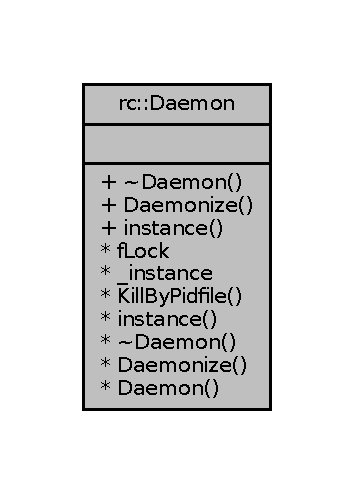
\includegraphics[width=170pt]{classrc_1_1Daemon__coll__graph}
\end{center}
\end{figure}
\subsection*{Public Member Functions}
\begin{Indent}{\bf Destruktor}\par
\begin{DoxyCompactItemize}
\item 
\hypertarget{classrc_1_1Daemon_a17b1d9a98318424c5b0893a5535b3f39}{{\bfseries $\sim$\+Daemon} (void)}\label{classrc_1_1Daemon_a17b1d9a98318424c5b0893a5535b3f39}

\end{DoxyCompactItemize}
\end{Indent}
\begin{Indent}{\bf Robo\+Cup als Systemdienst starten}\par
{\em 
\begin{DoxyParams}{Parameters}
{\em Dateipfad} & zur pidfile \\
\hline
{\em Dateipfad} & zur lockfile \\
\hline
{\em Name} & des non-\/root users unter welchem der Dienst laufen soll (D\+E\+A\+K\+T\+I\+V\+I\+E\+R\+T!) \\
\hline
\end{DoxyParams}

\begin{DoxyRetVals}{Return values}
{\em true,wenn} & der Dienst (fork(...)) erfolgreich war, sonst false \\
\hline
\end{DoxyRetVals}
}\begin{DoxyCompactItemize}
\item 
\hypertarget{classrc_1_1Daemon_a53ac269d47da15e64060e95c9d940326}{bool {\bfseries Daemonize} (std\+::string pidfile, std\+::string lockfile, std\+::string user)}\label{classrc_1_1Daemon_a53ac269d47da15e64060e95c9d940326}

\end{DoxyCompactItemize}
\end{Indent}
\subsection*{Static Public Member Functions}
\begin{Indent}{\bf Instanz der Singleton-\/ Klasse holen}\par
{\em 
\begin{DoxyRetVals}{Return values}
{\em Daemon-\/} & Objekt \\
\hline
\end{DoxyRetVals}
}\begin{DoxyCompactItemize}
\item 
\hypertarget{classrc_1_1Daemon_aa2428f2ddc48f857a3322da05d3c4b61}{static \hyperlink{classrc_1_1Daemon}{Daemon} $\ast$ {\bfseries instance} (void)}\label{classrc_1_1Daemon_aa2428f2ddc48f857a3322da05d3c4b61}

\end{DoxyCompactItemize}
\end{Indent}
\subsection*{Robo\+Cup Systemdienst beenden}
\label{_amgrp53b79b5f913ccbd72023be0cd06fb61f}%

\begin{DoxyParams}{Parameters}
{\em Dateipfad} & zur pidfile \\
\hline
{\em Dateipfad} & zur lockfile \\
\hline
\end{DoxyParams}

\begin{DoxyRetVals}{Return values}
{\em true,wenn} & der Dienst erfolgreich beendet werden konnte, sonst false \\
\hline
\end{DoxyRetVals}
\begin{DoxyCompactItemize}
\item 
\hypertarget{classrc_1_1Daemon_ae302feb46ccb0fc79c585082036328ba}{static bool {\bfseries Kill\+By\+Pidfile} (std\+::string pidfile, std\+::string lockfile)}\label{classrc_1_1Daemon_ae302feb46ccb0fc79c585082036328ba}

\end{DoxyCompactItemize}


\subsection{Detailed Description}
Klasse zum starten der Anwendung als Systemdienst 

The documentation for this class was generated from the following files\+:\begin{DoxyCompactItemize}
\item 
src/\hyperlink{RC__Daemon_8hpp}{R\+C\+\_\+\+Daemon.\+hpp}\item 
src/R\+C\+\_\+\+Daemon.\+cpp\end{DoxyCompactItemize}

\hypertarget{structrc_1_1processed__image}{\section{rc\+:\+:processed\+\_\+image Struct Reference}
\label{structrc_1_1processed__image}\index{rc\+::processed\+\_\+image@{rc\+::processed\+\_\+image}}
}


{\ttfamily \#include $<$R\+C\+\_\+\+Detector.\+hpp$>$}



Collaboration diagram for rc\+:\+:processed\+\_\+image\+:\nopagebreak
\begin{figure}[H]
\begin{center}
\leavevmode
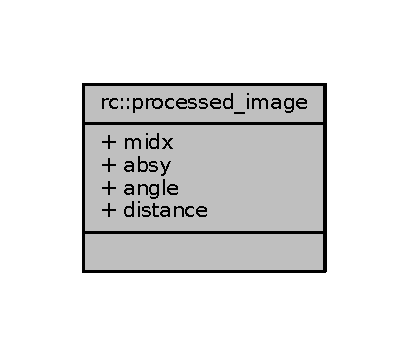
\includegraphics[width=196pt]{structrc_1_1processed__image__coll__graph}
\end{center}
\end{figure}
\subsection*{Public Attributes}
\begin{DoxyCompactItemize}
\item 
float \hyperlink{structrc_1_1processed__image_a0213f6e61795e2dbcaa500885554dbde}{midx}
\item 
float \hyperlink{structrc_1_1processed__image_a3885be6e15744069afb4b429777497fa}{absy}
\item 
float \hyperlink{structrc_1_1processed__image_ac17fea85630583e2cf1de55b89334e4f}{angle}
\item 
float \hyperlink{structrc_1_1processed__image_a6f90b2318450001568fcc112e294f8df}{distance}
\end{DoxyCompactItemize}


\subsection{Detailed Description}
wichtige Informationen eines bearbeiteten Bildes in dieser Struktur speichern 

\subsection{Member Data Documentation}
\hypertarget{structrc_1_1processed__image_a3885be6e15744069afb4b429777497fa}{\index{rc\+::processed\+\_\+image@{rc\+::processed\+\_\+image}!absy@{absy}}
\index{absy@{absy}!rc\+::processed\+\_\+image@{rc\+::processed\+\_\+image}}
\subsubsection[{absy}]{\setlength{\rightskip}{0pt plus 5cm}float rc\+::processed\+\_\+image\+::absy}}\label{structrc_1_1processed__image_a3885be6e15744069afb4b429777497fa}
Y-\/\+Koordinate (Y-\/\+Koordinate entspricht Y-\/\+Koordinate im Urpsrungsbild) \hypertarget{structrc_1_1processed__image_ac17fea85630583e2cf1de55b89334e4f}{\index{rc\+::processed\+\_\+image@{rc\+::processed\+\_\+image}!angle@{angle}}
\index{angle@{angle}!rc\+::processed\+\_\+image@{rc\+::processed\+\_\+image}}
\subsubsection[{angle}]{\setlength{\rightskip}{0pt plus 5cm}float rc\+::processed\+\_\+image\+::angle}}\label{structrc_1_1processed__image_ac17fea85630583e2cf1de55b89334e4f}
Winkel des rotierenden Rechteckes \hypertarget{structrc_1_1processed__image_a6f90b2318450001568fcc112e294f8df}{\index{rc\+::processed\+\_\+image@{rc\+::processed\+\_\+image}!distance@{distance}}
\index{distance@{distance}!rc\+::processed\+\_\+image@{rc\+::processed\+\_\+image}}
\subsubsection[{distance}]{\setlength{\rightskip}{0pt plus 5cm}float rc\+::processed\+\_\+image\+::distance}}\label{structrc_1_1processed__image_a6f90b2318450001568fcc112e294f8df}
die (geschätzte!) Entfernung zur Kamera \hypertarget{structrc_1_1processed__image_a0213f6e61795e2dbcaa500885554dbde}{\index{rc\+::processed\+\_\+image@{rc\+::processed\+\_\+image}!midx@{midx}}
\index{midx@{midx}!rc\+::processed\+\_\+image@{rc\+::processed\+\_\+image}}
\subsubsection[{midx}]{\setlength{\rightskip}{0pt plus 5cm}float rc\+::processed\+\_\+image\+::midx}}\label{structrc_1_1processed__image_a0213f6e61795e2dbcaa500885554dbde}
X-\/\+Koordinate (X=0 entspricht Breite des Bildes geteilt durch 2) 

The documentation for this struct was generated from the following file\+:\begin{DoxyCompactItemize}
\item 
src/\hyperlink{RC__Detector_8hpp}{R\+C\+\_\+\+Detector.\+hpp}\end{DoxyCompactItemize}

\hypertarget{classrc_1_1Semaphore}{\section{rc\+:\+:Semaphore Class Reference}
\label{classrc_1_1Semaphore}\index{rc\+::\+Semaphore@{rc\+::\+Semaphore}}
}
\subsection*{Public Member Functions}
\begin{Indent}{\bf Semaphore Konstruktor}\par
{\em aktuelle Anzahl der Konsumeinheiten


\begin{DoxyParams}{Parameters}
{\em maximale} & Anzahl der Konsumeinheiten \\
\hline
\end{DoxyParams}
}\begin{DoxyCompactItemize}
\item 
\hypertarget{classrc_1_1Semaphore_a6260f609fc0499bf67a7e5c77198f746}{{\bfseries Semaphore} (unsigned int \+\_\+max\+Count)}\label{classrc_1_1Semaphore_a6260f609fc0499bf67a7e5c77198f746}

\end{DoxyCompactItemize}
\end{Indent}
\begin{Indent}{\bf Destruktor}\par
\begin{DoxyCompactItemize}
\item 
\hypertarget{classrc_1_1Semaphore_ad7bb5c31cb578f9fb68983a23bd6a3e7}{{\bfseries $\sim$\+Semaphore} (void)}\label{classrc_1_1Semaphore_ad7bb5c31cb578f9fb68983a23bd6a3e7}

\end{DoxyCompactItemize}
\end{Indent}
\begin{Indent}{\bf Alle aufrufenden Threads blockieren, bis `count` == 0 ist}\par
{\em Jeder Thread, der diese Methode aufruft, wird blockiert bis {\ttfamily count} == 0 ist }\begin{DoxyCompactItemize}
\item 
\hypertarget{classrc_1_1Semaphore_a0fe2e6a5966af9b2e03dc5f8ffd64aff}{void {\bfseries Synchronize} (void)}\label{classrc_1_1Semaphore_a0fe2e6a5966af9b2e03dc5f8ffd64aff}

\end{DoxyCompactItemize}
\end{Indent}


The documentation for this class was generated from the following file\+:\begin{DoxyCompactItemize}
\item 
src/\hyperlink{RC__Semaphore_8hpp}{R\+C\+\_\+\+Semaphore.\+hpp}\end{DoxyCompactItemize}

\hypertarget{classrc_1_1WebServer}{\section{rc\+:\+:Web\+Server Class Reference}
\label{classrc_1_1WebServer}\index{rc\+::\+Web\+Server@{rc\+::\+Web\+Server}}
}
\subsection*{Public Member Functions}
\begin{Indent}{\bf Standartkonstruktor}\par
\begin{DoxyCompactItemize}
\item 
\hypertarget{classrc_1_1WebServer_afe32b4a720bb672a01b7e290507ae33e}{{\bfseries Web\+Server} (int port, int image\+\_\+count)}\label{classrc_1_1WebServer_afe32b4a720bb672a01b7e290507ae33e}

\end{DoxyCompactItemize}
\end{Indent}
\subsection*{Destruktor}
\begin{DoxyCompactItemize}
\item 
\hypertarget{classrc_1_1WebServer_a6b3b77c3c9bcc9668d558cbe71b57c15}{{\bfseries $\sim$\+Web\+Server} ()}\label{classrc_1_1WebServer_a6b3b77c3c9bcc9668d558cbe71b57c15}

\item 
\hypertarget{classrc_1_1WebServer_a44df359fc4f9e5e3209bf5cfcbb22980}{bool {\bfseries start} ()}\label{classrc_1_1WebServer_a44df359fc4f9e5e3209bf5cfcbb22980}

\item 
\hypertarget{classrc_1_1WebServer_a06ae92d6dadbbfdc4289c31fbfab6624}{void {\bfseries stop} (void)}\label{classrc_1_1WebServer_a06ae92d6dadbbfdc4289c31fbfab6624}

\item 
\hypertarget{classrc_1_1WebServer_af66eaf683e6e29c3f5c0530025aef5f7}{void {\bfseries set\+Image} (int idx, cv\+::\+Mat \&src)}\label{classrc_1_1WebServer_af66eaf683e6e29c3f5c0530025aef5f7}

\item 
\hypertarget{classrc_1_1WebServer_afa3effc52a15f4bef40da8209502ac72}{cv\+::\+Mat {\bfseries get\+Image} (int idx)}\label{classrc_1_1WebServer_afa3effc52a15f4bef40da8209502ac72}

\item 
\hypertarget{classrc_1_1WebServer_a1f8551f408b09eb67a49d050f253ed1f}{size\+\_\+t {\bfseries get\+Frames} (void)}\label{classrc_1_1WebServer_a1f8551f408b09eb67a49d050f253ed1f}

\item 
\hypertarget{classrc_1_1WebServer_ab0807008779f05091bab37f158b65b34}{size\+\_\+t {\bfseries get\+Count} (void)}\label{classrc_1_1WebServer_ab0807008779f05091bab37f158b65b34}

\item 
\hypertarget{classrc_1_1WebServer_a877ed11cc160de9b56851dafe396d25a}{std\+::vector$<$ int $>$ \& {\bfseries get\+Flags} (void)}\label{classrc_1_1WebServer_a877ed11cc160de9b56851dafe396d25a}

\end{DoxyCompactItemize}


The documentation for this class was generated from the following files\+:\begin{DoxyCompactItemize}
\item 
src/\hyperlink{RC__WebServer_8hpp}{R\+C\+\_\+\+Web\+Server.\+hpp}\item 
src/R\+C\+\_\+\+Web\+Server.\+cpp\end{DoxyCompactItemize}

\hypertarget{classrc_1_1Window}{\section{rc\+:\+:Window Class Reference}
\label{classrc_1_1Window}\index{rc\+::\+Window@{rc\+::\+Window}}
}
\subsection*{Public Member Functions}
\begin{DoxyCompactItemize}
\item 
\hypertarget{classrc_1_1Window_a115530da5a987d8c241b0febc3cddc8f}{void {\bfseries stop} (void)}\label{classrc_1_1Window_a115530da5a987d8c241b0febc3cddc8f}

\item 
\hypertarget{classrc_1_1Window_aa34989ba0c08041b7e3bcc35125340ec}{void {\bfseries add\+Image} (enum image\+Type type, cv\+::\+Mat image)}\label{classrc_1_1Window_aa34989ba0c08041b7e3bcc35125340ec}

\item 
\hypertarget{classrc_1_1Window_a15681842c7ce0ee6b9201cfa973d2ac1}{void {\bfseries run} (void)}\label{classrc_1_1Window_a15681842c7ce0ee6b9201cfa973d2ac1}

\item 
\hypertarget{classrc_1_1Window_a7cb65cbb3741a7711631f66c46c7b039}{bool {\bfseries images\+Available} (void)}\label{classrc_1_1Window_a7cb65cbb3741a7711631f66c46c7b039}

\item 
\hypertarget{classrc_1_1Window_a3c221423c38f30757d042b2621f22894}{size\+\_\+t {\bfseries images\+Queue\+Size} ()}\label{classrc_1_1Window_a3c221423c38f30757d042b2621f22894}

\item 
\hypertarget{classrc_1_1Window_aac13c76846e47e026d66eaf4a52fcd57}{void {\bfseries set\+X\+Window} (bool enable\+Win, bool enable\+Fltrd)}\label{classrc_1_1Window_aac13c76846e47e026d66eaf4a52fcd57}

\item 
\hypertarget{classrc_1_1Window_abd9877b14cf84b02e7c6ea54c23bc082}{bool {\bfseries is\+X\+Window} (void)}\label{classrc_1_1Window_abd9877b14cf84b02e7c6ea54c23bc082}

\item 
\hypertarget{classrc_1_1Window_a01dcc54995ffd8c973423566b6734d44}{bool {\bfseries is\+X\+Window\+Fltrd} (void)}\label{classrc_1_1Window_a01dcc54995ffd8c973423566b6734d44}

\end{DoxyCompactItemize}


The documentation for this class was generated from the following files\+:\begin{DoxyCompactItemize}
\item 
src/\hyperlink{RC__Window_8hpp}{R\+C\+\_\+\+Window.\+hpp}\item 
src/R\+C\+\_\+\+Window.\+cpp\end{DoxyCompactItemize}

\chapter{File Documentation}
\hypertarget{RC__BlobDetector_8hpp}{\section{src/\+R\+C\+\_\+\+Blob\+Detector.hpp File Reference}
\label{RC__BlobDetector_8hpp}\index{src/\+R\+C\+\_\+\+Blob\+Detector.\+hpp@{src/\+R\+C\+\_\+\+Blob\+Detector.\+hpp}}
}
{\ttfamily \#include $<$raspicam/raspicam\+\_\+cv.\+h$>$}\\*
{\ttfamily \#include $<$opencv2/opencv.\+hpp$>$}\\*
{\ttfamily \#include $<$opencv2/highgui/highgui.\+hpp$>$}\\*
\subsection*{Classes}
\begin{DoxyCompactItemize}
\item 
struct \hyperlink{structrc_1_1processed__image}{rc\+::processed\+\_\+image}
\item 
class \hyperlink{classrc_1_1BlobDetector}{rc\+::\+Blob\+Detector}
\end{DoxyCompactItemize}
\subsection*{Enumerations}
\begin{DoxyCompactItemize}
\item 
enum {\bfseries robo\+Color} \{ {\bfseries R\+B\+\_\+\+Y\+E\+L\+L\+O\+W}, 
{\bfseries R\+B\+\_\+\+B\+L\+U\+E}
 \}
\end{DoxyCompactItemize}


\subsection{Detailed Description}
\begin{DoxyAuthor}{Author}
Toni Uhlig \href{mailto:matzeton@googlemail.com}{\tt matzeton@googlemail.\+com} 
\end{DoxyAuthor}
\begin{DoxyDate}{Date}
25.\+05.\+2016 
\end{DoxyDate}
\begin{DoxyVersion}{Version}
1.\+0 
\end{DoxyVersion}

\hypertarget{RC__BlobDetectorFactory_8hpp}{\section{src/\+R\+C\+\_\+\+Blob\+Detector\+Factory.hpp File Reference}
\label{RC__BlobDetectorFactory_8hpp}\index{src/\+R\+C\+\_\+\+Blob\+Detector\+Factory.\+hpp@{src/\+R\+C\+\_\+\+Blob\+Detector\+Factory.\+hpp}}
}
{\ttfamily \#include $<$iostream$>$}\\*
{\ttfamily \#include $<$ostream$>$}\\*
{\ttfamily \#include $<$raspicam/raspicam\+\_\+cv.\+h$>$}\\*
{\ttfamily \#include $<$thread$>$}\\*
{\ttfamily \#include $<$condition\+\_\+variable$>$}\\*
{\ttfamily \#include $<$atomic$>$}\\*
{\ttfamily \#include \char`\"{}R\+C\+\_\+\+Camera.\+hpp\char`\"{}}\\*
{\ttfamily \#include \char`\"{}R\+C\+\_\+\+Semaphore.\+hpp\char`\"{}}\\*
{\ttfamily \#include \char`\"{}R\+C\+\_\+\+Circular\+Buffer.\+hpp\char`\"{}}\\*
{\ttfamily \#include \char`\"{}R\+C\+\_\+\+Blob\+Detector.\+hpp\char`\"{}}\\*
\subsection*{Classes}
\begin{DoxyCompactItemize}
\item 
class \hyperlink{classrc_1_1BlobDetectorFactory}{rc\+::\+Blob\+Detector\+Factory}
\end{DoxyCompactItemize}
\subsection*{Namespaces}
\begin{DoxyCompactItemize}
\item 
 \hyperlink{namespacerc}{rc}
\end{DoxyCompactItemize}


\subsection{Detailed Description}
\begin{DoxyDate}{Date}
25.\+05.\+2016 
\end{DoxyDate}
\begin{DoxyAuthor}{Author}
Toni Uhlig \href{mailto:matzeton@googlemail.com}{\tt matzeton@googlemail.\+com} 
\end{DoxyAuthor}
\begin{DoxyVersion}{Version}
1.\+0 
\end{DoxyVersion}

\hypertarget{RC__Camera_8hpp}{\section{src/\+R\+C\+\_\+\+Camera.hpp File Reference}
\label{RC__Camera_8hpp}\index{src/\+R\+C\+\_\+\+Camera.\+hpp@{src/\+R\+C\+\_\+\+Camera.\+hpp}}
}


Eine Klasse zur Steuerung der Kamera und des Zwischenspeichers (Puffer)  


{\ttfamily \#include $<$raspicam/raspicam.\+h$>$}\\*
{\ttfamily \#include $<$raspicam/raspicam\+\_\+cv.\+h$>$}\\*
{\ttfamily \#include $<$raspicam/raspicamtypes.\+h$>$}\\*
{\ttfamily \#include \char`\"{}R\+C\+\_\+\+Circular\+Buffer.\+hpp\char`\"{}}\\*
\subsection*{Classes}
\begin{DoxyCompactItemize}
\item 
class \hyperlink{classrc_1_1Camera}{rc\+::\+Camera}
\end{DoxyCompactItemize}
\subsection*{Namespaces}
\begin{DoxyCompactItemize}
\item 
 \hyperlink{namespacerc}{rc}
\end{DoxyCompactItemize}


\subsection{Detailed Description}
Eine Klasse zur Steuerung der Kamera und des Zwischenspeichers (Puffer) 

\begin{DoxyDate}{Date}
25.\+05.\+2016 
\end{DoxyDate}
\begin{DoxyAuthor}{Author}
Toni Uhlig \href{mailto:matzeton@googlemail.com}{\tt matzeton@googlemail.\+com} Diese Klasse ermöglicht eine einfache Steuerung der Raspicam (mit Open\+C\+V Unterstützung). Dabei erbt \hyperlink{classrc_1_1Camera}{rc\+::\+Camera} von beiden Klassen {\ttfamily protected}. Für mehr Informationen\+: \href{https://de.wikibooks.org/wiki/C%2B%2B-Programmierung:_Vererbung}{\tt https\+://de.\+wikibooks.\+org/wiki/\+C\%2\+B\%2\+B-\/\+Programmierung\+:\+\_\+\+Vererbung} 
\end{DoxyAuthor}

\hypertarget{RC__CircularBuffer_8hpp}{\section{src/\+R\+C\+\_\+\+Circular\+Buffer.hpp File Reference}
\label{RC__CircularBuffer_8hpp}\index{src/\+R\+C\+\_\+\+Circular\+Buffer.\+hpp@{src/\+R\+C\+\_\+\+Circular\+Buffer.\+hpp}}
}
{\ttfamily \#include $<$iostream$>$}\\*
{\ttfamily \#include $<$vector$>$}\\*
{\ttfamily \#include $<$mutex$>$}\\*
{\ttfamily \#include $<$time.\+h$>$}\\*
\subsection*{Classes}
\begin{DoxyCompactItemize}
\item 
struct \hyperlink{structrc_1_1cbElement}{rc\+::cb\+Element$<$ T $>$}
\item 
class \hyperlink{classrc_1_1CircularBuffer}{rc\+::\+Circular\+Buffer$<$ T $>$}
\end{DoxyCompactItemize}


\subsection{Detailed Description}
\begin{DoxyAuthor}{Author}
Toni Uhlig \href{mailto:matzeton@googlemail.com}{\tt matzeton@googlemail.\+com} 
\end{DoxyAuthor}
\begin{DoxyDate}{Date}
24.\+05.\+2016 
\end{DoxyDate}
\begin{DoxyVersion}{Version}
1.\+0 
\end{DoxyVersion}

\hypertarget{RC__Daemon_8hpp}{\section{src/\+R\+C\+\_\+\+Daemon.hpp File Reference}
\label{RC__Daemon_8hpp}\index{src/\+R\+C\+\_\+\+Daemon.\+hpp@{src/\+R\+C\+\_\+\+Daemon.\+hpp}}
}
{\ttfamily \#include $<$string$>$}\\*
\subsection*{Classes}
\begin{DoxyCompactItemize}
\item 
class \hyperlink{classrc_1_1Daemon}{rc\+::\+Daemon}
\end{DoxyCompactItemize}
\subsection*{Functions}
\begin{Indent}{\bf Prüfung ob Dienst bereits terminiert wird/wurde}\par
{\em 
\begin{DoxyRetVals}{Return values}
{\em true,wenn} & Dienst bereits terminiert, sonst false \\
\hline
\end{DoxyRetVals}
}\begin{DoxyCompactItemize}
\item 
bool {\bfseries rc\+::is\+Daemon\+Terminate} (void)
\end{DoxyCompactItemize}
\end{Indent}
\begin{Indent}{\bf Anwendungsstart abschließen}\par
{\em Diese Routine sollte nach der Initialisierung aufgerufen werden. }\begin{DoxyCompactItemize}
\item 
\hypertarget{namespacerc_ad7301d689ad53a4f46b1f4c14c72e97e}{void {\bfseries rc\+::start\+Up\+Done} (void)}\label{namespacerc_ad7301d689ad53a4f46b1f4c14c72e97e}

\end{DoxyCompactItemize}
\end{Indent}
\begin{Indent}{\bf Reaktion auf Systemspez. Signale festlegen}\par
\begin{DoxyCompactItemize}
\item 
\hypertarget{namespacerc_a394315bf537365634692ccb2bc32b287}{void {\bfseries rc\+::set\+Signals} (void)}\label{namespacerc_a394315bf537365634692ccb2bc32b287}

\end{DoxyCompactItemize}
\end{Indent}


\subsection{Detailed Description}
\begin{DoxyAuthor}{Author}
Toni Uhlig \href{mailto:matzeton@googlemail.com}{\tt matzeton@googlemail.\+com} 
\end{DoxyAuthor}
\begin{DoxyDate}{Date}
16.\+07.\+2016 
\end{DoxyDate}
\begin{DoxyVersion}{Version}
1.\+0 
\end{DoxyVersion}

\hypertarget{RC__Main_8cpp}{\section{src/\+R\+C\+\_\+\+Main.cpp File Reference}
\label{RC__Main_8cpp}\index{src/\+R\+C\+\_\+\+Main.\+cpp@{src/\+R\+C\+\_\+\+Main.\+cpp}}
}


Initialisierung, Parameter auswerten, Einstellungen setzen.  


{\ttfamily \#include $<$unistd.\+h$>$}\\*
{\ttfamily \#include $<$stdint.\+h$>$}\\*
{\ttfamily \#include $<$ctime$>$}\\*
{\ttfamily \#include $<$iostream$>$}\\*
{\ttfamily \#include $<$iomanip$>$}\\*
{\ttfamily \#include $<$raspicam/raspicam\+\_\+cv.\+h$>$}\\*
{\ttfamily \#include \char`\"{}R\+C\+\_\+\+Daemon.\+hpp\char`\"{}}\\*
{\ttfamily \#include \char`\"{}R\+C\+\_\+\+Blob\+Detector\+Factory.\+hpp\char`\"{}}\\*
\subsection*{Classes}
\begin{DoxyCompactItemize}
\item 
struct \hyperlink{structcmd__opts}{cmd\+\_\+opts}
\end{DoxyCompactItemize}
\subsection*{Macros}
\begin{DoxyCompactItemize}
\item 
\#define \hyperlink{RC__Main_8cpp_af5fe208f8640c8c789a4d5d5b8ad47f5}{P\+I\+D\+F\+I\+L\+E}~\char`\"{}/var/run/robocup.\+pid\char`\"{}
\item 
\#define \hyperlink{RC__Main_8cpp_a551ae9e7796a78ff54bc98eef4e74498}{L\+O\+C\+K\+F\+I\+L\+E}~\char`\"{}/var/lock/robocup.\+lock\char`\"{}
\item 
\#define \hyperlink{RC__Main_8cpp_acd9f5e44663c48631109f64baca83ea7}{C\+H\+U\+S\+E\+R}~\char`\"{}robocup\char`\"{}
\item 
\#define \hyperlink{RC__Main_8cpp_a1a2717f1b81aff0aeaa7461a104df0e4}{U\+N\+I\+M\+P\+L\+E\+M\+E\+N\+T\+E\+D}(feature)~\{ fprintf(stderr, \char`\"{}\%s\+: feature not implemented (\%s)\textbackslash{}n\char`\"{}, argv\mbox{[}0\mbox{]}, feature); exit(1); \}
\end{DoxyCompactItemize}
\subsection*{Functions}
\begin{Indent}{\bf Kommandozeilenhilfe}\par
{\em Eine kurze Übersicht über alle verfügbaren Konfigurationsvariablen }\end{Indent}
\begin{Indent}{\bf `main` Funktion}\par
{\em Diese wird vom Betriebssystem während des Programmstartes als Einsprungspunkt genutzt


\begin{DoxyRetVals}{Return values}
{\em ganzzahliger} & Rückgabewert der z.\+B. auf der Shell ausgewertet werden kann \\
\hline
\end{DoxyRetVals}
}\begin{DoxyCompactItemize}
\item 
\hypertarget{RC__Main_8cpp_a3c04138a5bfe5d72780bb7e82a18e627}{int {\bfseries main} (int argc, char $\ast$$\ast$argv)}\label{RC__Main_8cpp_a3c04138a5bfe5d72780bb7e82a18e627}

\end{DoxyCompactItemize}
\end{Indent}


\subsection{Detailed Description}
Initialisierung, Parameter auswerten, Einstellungen setzen. 

\begin{DoxyDate}{Date}
20.\+05.\+2016 
\end{DoxyDate}
\begin{DoxyAuthor}{Author}
Toni Uhlig \href{mailto:matzeton@googlemail.com}{\tt matzeton@googlemail.\+com} 
\end{DoxyAuthor}


\subsection{Macro Definition Documentation}
\hypertarget{RC__Main_8cpp_acd9f5e44663c48631109f64baca83ea7}{\index{R\+C\+\_\+\+Main.\+cpp@{R\+C\+\_\+\+Main.\+cpp}!C\+H\+U\+S\+E\+R@{C\+H\+U\+S\+E\+R}}
\index{C\+H\+U\+S\+E\+R@{C\+H\+U\+S\+E\+R}!R\+C\+\_\+\+Main.\+cpp@{R\+C\+\_\+\+Main.\+cpp}}
\subsubsection[{C\+H\+U\+S\+E\+R}]{\setlength{\rightskip}{0pt plus 5cm}\#define C\+H\+U\+S\+E\+R~\char`\"{}robocup\char`\"{}}}\label{RC__Main_8cpp_acd9f5e44663c48631109f64baca83ea7}
Standartuser, um nicht benötigte Privilegien zu \char`\"{}droppen\char`\"{} (daemon Modus) \hypertarget{RC__Main_8cpp_a551ae9e7796a78ff54bc98eef4e74498}{\index{R\+C\+\_\+\+Main.\+cpp@{R\+C\+\_\+\+Main.\+cpp}!L\+O\+C\+K\+F\+I\+L\+E@{L\+O\+C\+K\+F\+I\+L\+E}}
\index{L\+O\+C\+K\+F\+I\+L\+E@{L\+O\+C\+K\+F\+I\+L\+E}!R\+C\+\_\+\+Main.\+cpp@{R\+C\+\_\+\+Main.\+cpp}}
\subsubsection[{L\+O\+C\+K\+F\+I\+L\+E}]{\setlength{\rightskip}{0pt plus 5cm}\#define L\+O\+C\+K\+F\+I\+L\+E~\char`\"{}/var/lock/robocup.\+lock\char`\"{}}}\label{RC__Main_8cpp_a551ae9e7796a78ff54bc98eef4e74498}
Standartpfad für Sperr-\/ Datei (daemon Modus) \hypertarget{RC__Main_8cpp_af5fe208f8640c8c789a4d5d5b8ad47f5}{\index{R\+C\+\_\+\+Main.\+cpp@{R\+C\+\_\+\+Main.\+cpp}!P\+I\+D\+F\+I\+L\+E@{P\+I\+D\+F\+I\+L\+E}}
\index{P\+I\+D\+F\+I\+L\+E@{P\+I\+D\+F\+I\+L\+E}!R\+C\+\_\+\+Main.\+cpp@{R\+C\+\_\+\+Main.\+cpp}}
\subsubsection[{P\+I\+D\+F\+I\+L\+E}]{\setlength{\rightskip}{0pt plus 5cm}\#define P\+I\+D\+F\+I\+L\+E~\char`\"{}/var/run/robocup.\+pid\char`\"{}}}\label{RC__Main_8cpp_af5fe208f8640c8c789a4d5d5b8ad47f5}
Standartpfad für die Prozess\+I\+D-\/ Datei (daemon Modus) \hypertarget{RC__Main_8cpp_a1a2717f1b81aff0aeaa7461a104df0e4}{\index{R\+C\+\_\+\+Main.\+cpp@{R\+C\+\_\+\+Main.\+cpp}!U\+N\+I\+M\+P\+L\+E\+M\+E\+N\+T\+E\+D@{U\+N\+I\+M\+P\+L\+E\+M\+E\+N\+T\+E\+D}}
\index{U\+N\+I\+M\+P\+L\+E\+M\+E\+N\+T\+E\+D@{U\+N\+I\+M\+P\+L\+E\+M\+E\+N\+T\+E\+D}!R\+C\+\_\+\+Main.\+cpp@{R\+C\+\_\+\+Main.\+cpp}}
\subsubsection[{U\+N\+I\+M\+P\+L\+E\+M\+E\+N\+T\+E\+D}]{\setlength{\rightskip}{0pt plus 5cm}\#define U\+N\+I\+M\+P\+L\+E\+M\+E\+N\+T\+E\+D(
\begin{DoxyParamCaption}
\item[{}]{feature}
\end{DoxyParamCaption}
)~\{ fprintf(stderr, \char`\"{}\%s\+: feature not implemented (\%s)\textbackslash{}n\char`\"{}, argv\mbox{[}0\mbox{]}, feature); exit(1); \}}}\label{RC__Main_8cpp_a1a2717f1b81aff0aeaa7461a104df0e4}
Dieses Feature ist zur Zeit nicht im \char`\"{}binary\char`\"{} enthalten. Um das Feature zu integrieren muss das Projekt mit {\ttfamily cmake} bzw. {\ttfamily ccmake} neu kofniguriert/kompiliert/gelinkt werden. 
\hypertarget{RC__Semaphore_8hpp}{\section{src/\+R\+C\+\_\+\+Semaphore.hpp File Reference}
\label{RC__Semaphore_8hpp}\index{src/\+R\+C\+\_\+\+Semaphore.\+hpp@{src/\+R\+C\+\_\+\+Semaphore.\+hpp}}
}
{\ttfamily \#include $<$iostream$>$}\\*
{\ttfamily \#include $<$thread$>$}\\*
{\ttfamily \#include $<$mutex$>$}\\*
{\ttfamily \#include $<$condition\+\_\+variable$>$}\\*
\subsection*{Classes}
\begin{DoxyCompactItemize}
\item 
class \hyperlink{classrc_1_1Semaphore}{rc\+::\+Semaphore}
\end{DoxyCompactItemize}


\subsection{Detailed Description}
\begin{DoxyAuthor}{Author}
Toni Uhlig \href{mailto:matzeton@googlemail.com}{\tt matzeton@googlemail.\+com} 
\end{DoxyAuthor}
\begin{DoxyDate}{Date}
16.\+07.\+2016 
\end{DoxyDate}
\begin{DoxyVersion}{Version}
1.\+0 
\end{DoxyVersion}

\hypertarget{RC__WebServer_8hpp}{\section{src/\+R\+C\+\_\+\+Web\+Server.hpp File Reference}
\label{RC__WebServer_8hpp}\index{src/\+R\+C\+\_\+\+Web\+Server.\+hpp@{src/\+R\+C\+\_\+\+Web\+Server.\+hpp}}
}
{\ttfamily \#include $<$thread$>$}\\*
{\ttfamily \#include $<$mutex$>$}\\*
{\ttfamily \#include $<$raspicam/raspicam\+\_\+cv.\+h$>$}\\*
{\ttfamily \#include $<$opencv2/opencv.\+hpp$>$}\\*
{\ttfamily \#include $<$microhttpd.\+h$>$}\\*
\subsection*{Classes}
\begin{DoxyCompactItemize}
\item 
class \hyperlink{classrc_1_1WebServer}{rc\+::\+Web\+Server}
\end{DoxyCompactItemize}


\subsection{Detailed Description}
\begin{DoxyAuthor}{Author}
Toni Uhlig \href{mailto:matzeton@googlemail.com}{\tt matzeton@googlemail.\+com} 
\end{DoxyAuthor}
\begin{DoxyDate}{Date}
20.\+08.\+2016 
\end{DoxyDate}
\begin{DoxyVersion}{Version}
1.\+0 
\end{DoxyVersion}

\hypertarget{RC__Window_8hpp}{\section{src/\+R\+C\+\_\+\+Window.hpp File Reference}
\label{RC__Window_8hpp}\index{src/\+R\+C\+\_\+\+Window.\+hpp@{src/\+R\+C\+\_\+\+Window.\+hpp}}
}
{\ttfamily \#include $<$iostream$>$}\\*
{\ttfamily \#include $<$raspicam/raspicam\+\_\+cv.\+h$>$}\\*
{\ttfamily \#include $<$condition\+\_\+variable$>$}\\*
{\ttfamily \#include $<$thread$>$}\\*
{\ttfamily \#include $<$atomic$>$}\\*
{\ttfamily \#include $<$queue$>$}\\*
\subsection*{Classes}
\begin{DoxyCompactItemize}
\item 
class \hyperlink{classrc_1_1Window}{rc\+::\+Window}
\end{DoxyCompactItemize}


\subsection{Detailed Description}
\begin{DoxyAuthor}{Author}
Toni Uhlig \href{mailto:matzeton@googlemail.com}{\tt matzeton@googlemail.\+com} 
\end{DoxyAuthor}
\begin{DoxyDate}{Date}
25.\+05.\+2016 
\end{DoxyDate}
\begin{DoxyVersion}{Version}
1.\+0 
\end{DoxyVersion}

%--- End generated contents ---

% Index
\newpage
\phantomsection
\addcontentsline{toc}{chapter}{Index}
\printindex

\end{document}
